\section{Resultados}

Todos los resultados pertenecen al contrato de cinco salidas y al mismo corpus final. El conjunto de validación determina candidato, calibradores, umbrales y política; el test solo estima el desempeño del artefacto ya congelado.

\subsection{Comparación global en el conjunto de validación}

La comparación contiene 28 candidatos individuales y cinco reglas base de ensemble; la actualización añade la optimización simétrica de los ensembles suave y duro dentro del mismo flujo. Qwen3--LoRA es el mejor individuo y el ensemble suave optimizado ocupa el primer lugar actual. Su evaluación anidada obtiene BA 0,8366 y macro-AUPRC 0,5506; frente a Qwen OOF, las diferencias descriptivas son $+0,0052$ y $+0,0349$. Las Tablas~\ref{tab:tipos} y~\ref{tab:ensembles} presentan los resultados vigentes y el hardware empleado, sin intercalar un segundo ranking histórico.

\begin{table}[t]
\centering
\caption{Mejor candidato por tipo en el conjunto de validación OOF. Fuente: elaboración propia a partir de los registros de la comparación integrada.}
\label{tab:tipos}
\footnotesize
\resizebox{\columnwidth}{!}{%
\begin{tabular}{@{}lrrrrr@{}}
\toprule
\textbf{Tipo} & \textbf{BA} & \textbf{AUPRC} & \textbf{F1} & \textbf{FNR} & \textbf{FPR} \\
\midrule
Clásico, logística $C=0,5$\textsuperscript{a} & 0,80 & 0,48 & 0,50 & 0,18 & 0,22 \\
Transformer, cascada segura\textsuperscript{b} & 0,82 & 0,45 & 0,52 & 0,16 & 0,21 \\
Qwen3--LoRA\textsuperscript{c} & 0,83 & 0,52 & 0,55 & 0,17 & 0,17 \\
\textbf{Ensemble suave optimizado}\textsuperscript{d} & \textbf{0,837} & \textbf{0,551} & \textbf{0,562} & \textbf{0,150} & 0,177 \\
\bottomrule
\end{tabular}%
}
\begin{minipage}{.98\columnwidth}\vspace{1mm}\footnotesize
\emph{Nota:} AUPRC y F1 son promedios macro de los cuatro daños; BA, FNR y FPR corresponden a \texttt{ANY\_DAMAGE} OOF a cobertura completa. Hardware: \textsuperscript{a}CPU Intel64, cuatro hilos; \textsuperscript{b}NVIDIA L4 de 23~GiB; \textsuperscript{c}NVIDIA A100-SXM4 de 40~GB; \textsuperscript{d}CPU AMD Ryzen 7 8845HS. La Tabla~\ref{tab:hardware_tiempos} detalla las tareas y los tiempos.
\end{minipage}
\end{table}

Las siete variantes usan los mismos tres miembros y se reevalúan con calibración interna idéntica (Tabla~\ref{tab:ensembles}). La optimización cambia el resultado: el ensemble suave aprendido pasa al rango uno. El ensemble ponderado heurístico conserva mayor macro-AUPRC y F1, pero tiene BA y riesgo inferiores según el orden predeclarado. Los ensembles de unión e intersección carecen de coeficientes; por eso solo se recalibran.

\begin{table}[t]
\centering
\caption{Comparación de las siete variantes de ensemble mediante validación anidada. Fuente: elaboración propia a partir del cuaderno reproducible de optimización.}
\label{tab:ensembles}
\footnotesize
\resizebox{\columnwidth}{!}{%
\begin{tabular}{@{}lrrrr@{}}
\toprule
\textbf{Regla} & \textbf{BA} & $\boldsymbol{R_{0,67}}$ & \textbf{Macro-AUPRC} & \textbf{Macro-F1} \\
\midrule
\textbf{Ensemble suave optimizado} & \textbf{0,8366} & \textbf{0,1587} & 0,5506 & 0,5618 \\
Ensemble ponderado AUPRC & 0,8360 & 0,1612 & \textbf{0,5614} & 0,5675 \\
Ensemble de unión & 0,8334 & 0,1684 & 0,5369 & 0,5621 \\
Ensemble de promedio suave & 0,8328 & 0,1673 & 0,5604 & \textbf{0,5703} \\
Ensemble duro optimizado & 0,8272 & 0,1731 & 0,4547 & 0,5584 \\
Ensemble de mayoría dura & 0,8272 & 0,1731 & 0,4415 & 0,5638 \\
Ensemble de intersección & 0,8149 & 0,1887 & 0,5131 & 0,5373 \\
\bottomrule
\end{tabular}%
}
\end{table}

Los coeficientes congelados del ganador se muestran en la Tabla~\ref{tab:pesos_ganador}; se aplican a probabilidades ya calibradas por miembro y suman uno.

\begin{table}[t]
\centering
\caption{Coeficientes del único ensemble ganador actual. Fuente: elaboración propia a partir del ajuste final sobre el conjunto de validación.}
\label{tab:pesos_ganador}
\footnotesize
\begin{tabular}{@{}lr@{}}
\toprule
\textbf{Miembro} & $\boldsymbol{w_m}$ \\
\midrule
Regresión logística $C=0,5$ & 0,10 \\
Cascada E5 segura & 0,65 \\
Qwen3--LoRA & 0,25 \\
\midrule
Suma & 1,00 \\
\bottomrule
\end{tabular}
\end{table}

\subsection{Frontera de Pareto e incertidumbre}

El retador más cercano es el ensemble ponderado por AUPRC. En 2\,000 réplicas pareadas por video, la diferencia de BA entre el ganador y el retador es 0,00059, con IC95\% $[-0,00367,\,0,00509]$ y $p=0,80$ sin corrección. El intervalo incluye cero. La regla lexicográfica selecciona \texttt{ensemble\_soft\_optimized} como único ganador, pero el contraste no demuestra superioridad estadística. Los pesos suaves también varían entre los pliegues externos, sobre todo el peso del Transformer; el Apéndice~\ref{app:ensemble} cuantifica esa variación.

\subsection{Desempeño del ensemble por salida}

Con los calibradores de despliegue ajustados en todo el conjunto de validación, el ensemble optimizado alcanza macro-AUPRC 0,55 y macro-F1 0,55 sobre los cuatro daños (Tabla~\ref{tab:ensemble_categorias}). Contenido sexual obtiene el mayor F1 (0,63) y género/identidad el menor (0,42). Estos valores descriptivos del ajuste final no reemplazan la estimación anidada usada para seleccionar.

\begin{table}[t]
\centering
\caption{Desempeño del ensemble seleccionado por categoría en el conjunto de validación. Fuente: elaboración propia a partir del ajuste final.}
\label{tab:ensemble_categorias}
\footnotesize
\begin{tabular}{@{}lrrrrr@{}}
\toprule
\textbf{Salida} & \textbf{Soporte} & \textbf{AUPRC} & \textbf{Prec.} & \textbf{Rec.} & \textbf{F1} \\
\midrule
\texttt{SEGURO} & 8\,480 & 0,98 & 0,89 & 0,95 & 0,92 \\
\Rac & 382 & 0,55 & 0,51 & 0,69 & 0,59 \\
\Gen & 374 & 0,37 & 0,36 & 0,52 & 0,42 \\
\Ame & 1\,146 & 0,60 & 0,59 & 0,53 & 0,56 \\
\Sex & 633 & 0,68 & 0,73 & 0,56 & 0,63 \\
\bottomrule
\end{tabular}
\end{table}

Los mejores candidatos dependen de la categoría. Qwen3--LoRA con contexto 256 lidera AUPRC en racismo (0,57) y género/identidad (0,40); el ensemble ponderado lidera acoso/amenaza (0,61) y \texttt{SEGURO} (0,97); el ensemble de promedio simple lidera contenido sexual (0,69). La Fig.~\ref{fig:categorias_final} muestra AUPRC y F1 de esos especialistas. El detalle de ganadores por métrica se conserva en el Apéndice~\ref{app:resultados}. Para operación se mantiene un único ensemble global, evitando reglas por categoría elegidas \emph{post hoc}.

\begin{figure*}[t]
\centering
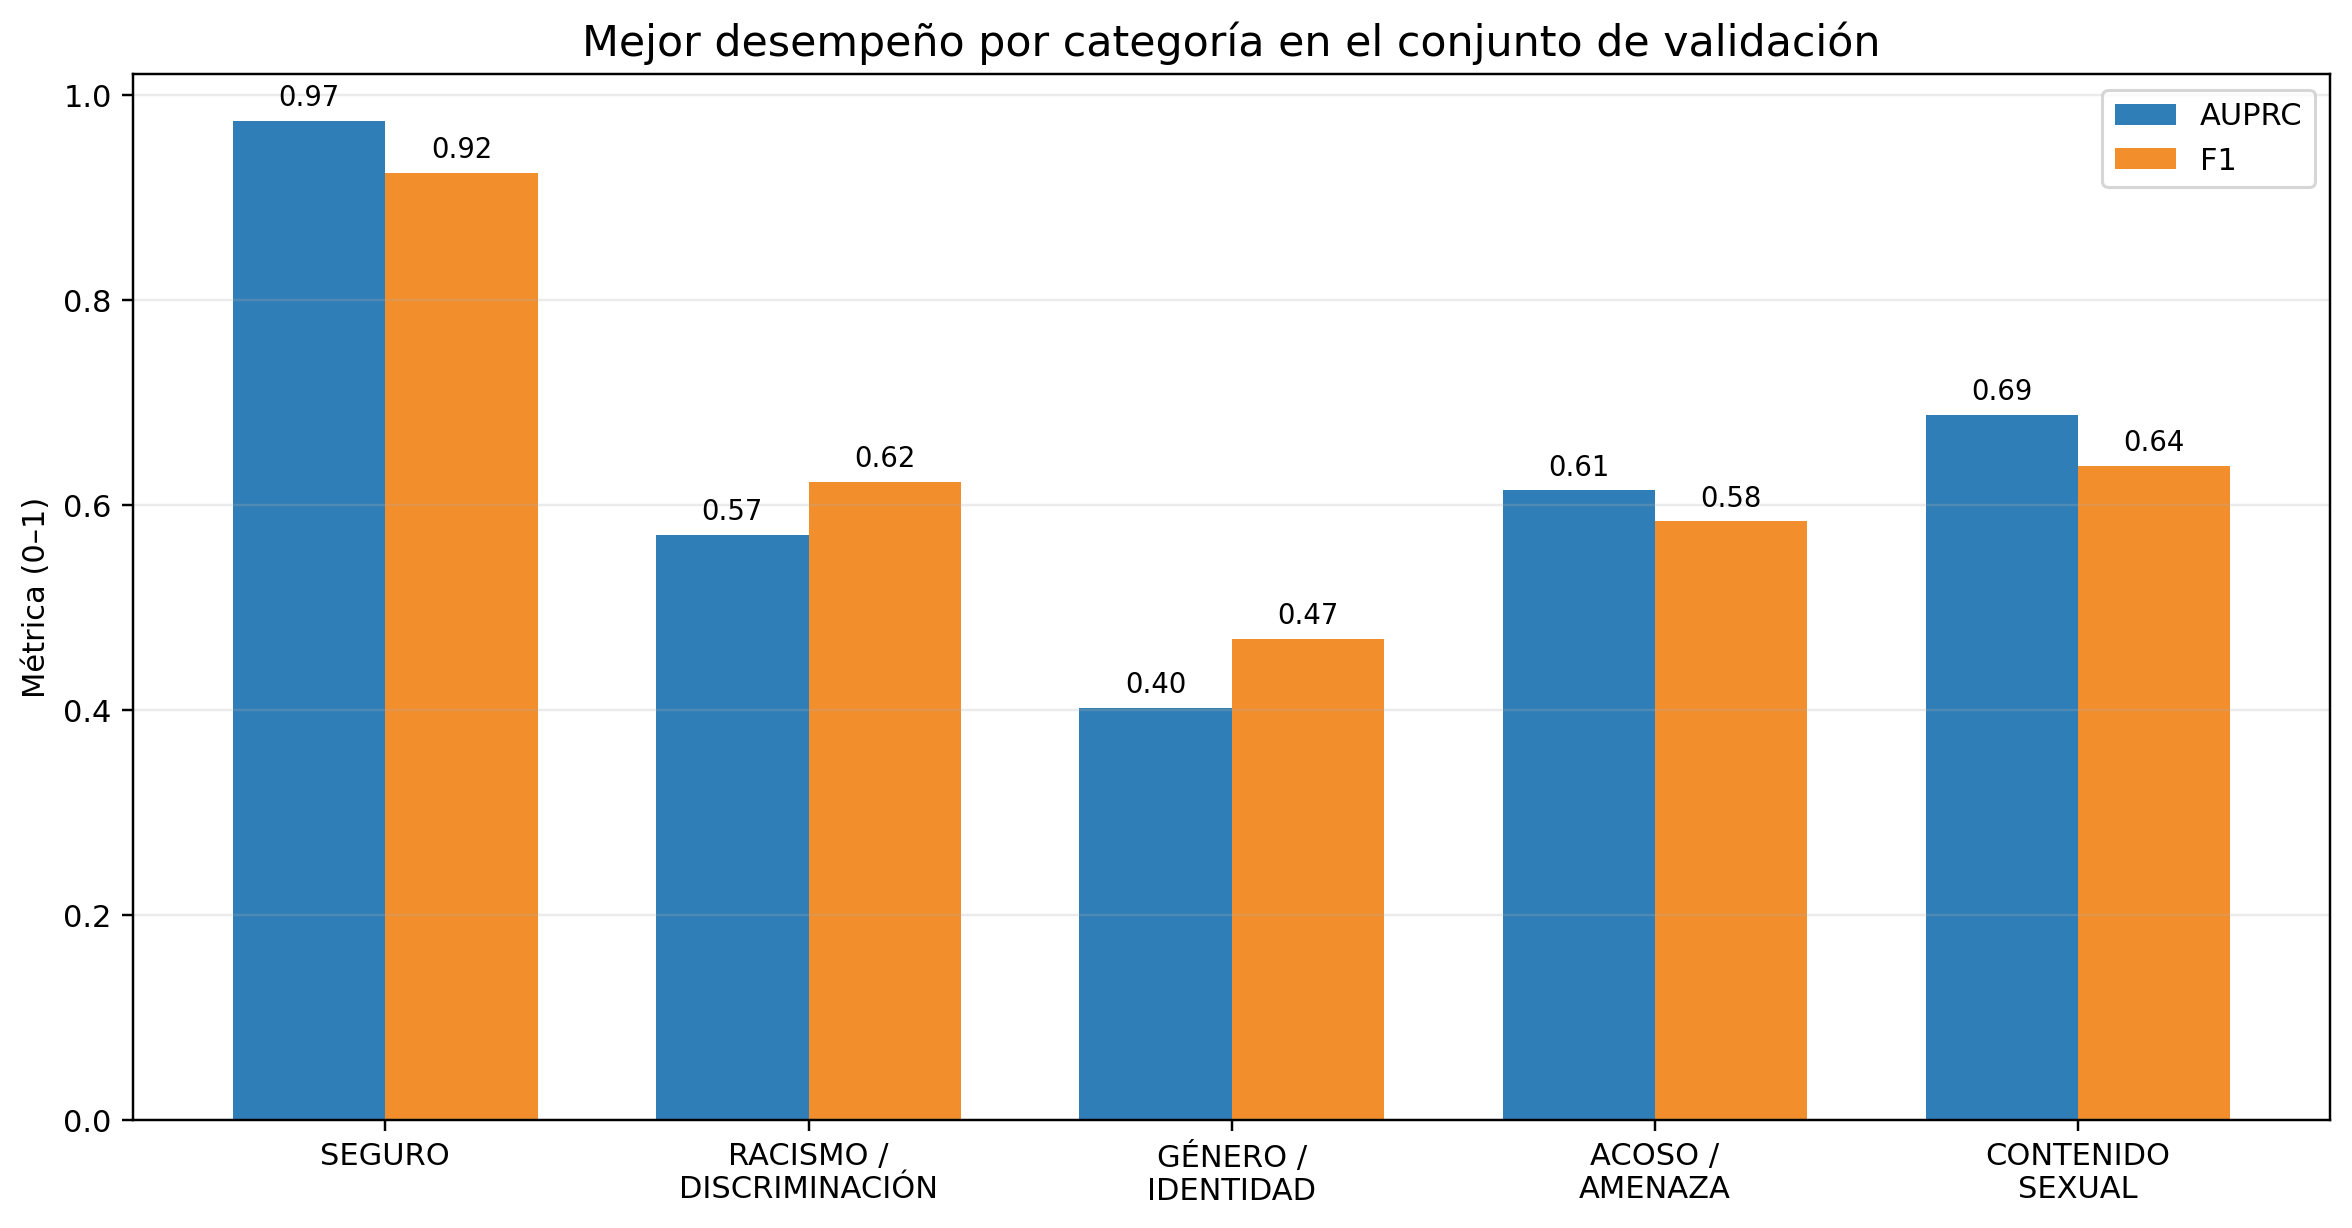
\includegraphics[width=.88\textwidth]{figuras/seleccion_por_categoria_conjunto_validacion.png}
\caption{Mejor desempeño por categoría en el conjunto de validación entre candidatos que superan la salvaguarda global. Fuente: elaboración propia a partir de la comparación integrada.}
\label{fig:categorias_final}
\end{figure*}

\subsection{Apertura única de test natural}

El test contiene 22\,684 chunks, 1\,802 con algún daño (7,9\%). La compuerta optimizada identifica 1\,611 y omite 191: sensibilidad 0,894, especificidad 0,798 y BA 0,846. Frente al ensemble de promedio simple, la BA cambia solo $+0,00004$; disminuyen los falsos positivos (4\,466 a 4\,221), pero aumentan los falsos negativos (170 a 191). Estas cifras no se usaron para recalibrar ni volver a escoger el modelo.

En la tarea multietiqueta completa, la macro-AUPRC de daños es 0,412 y la macro-F1 0,423. La caída respecto de la vista 4:1 se concentra en precisión y AUPRC porque el test natural contiene 12 seguros por daño; la sensibilidad y la BA de la compuerta se mantienen. La Tabla~\ref{tab:test_categorias} localiza la variación por salida. El contraste entre ambas vistas confirma que AUPRC debe interpretarse junto con la prevalencia \cite{tonneau2024naijahate}.

\begin{table}[t]
\centering
\caption{Desempeño por salida del ensemble optimizado en el test natural. Fuente: elaboración propia a partir de la apertura única de test.}
\label{tab:test_categorias}
\footnotesize
\begin{tabular}{@{}lrrrrr@{}}
\toprule
\textbf{Salida} & \textbf{Soporte} & \textbf{AUPRC} & \textbf{Prec.} & \textbf{Rec.} & \textbf{F1} \\
\midrule
\texttt{SEGURO} & 20\,882 & 0,99 & 0,96 & 0,95 & 0,95 \\
\Rac & 308 & 0,36 & 0,25 & 0,65 & 0,36 \\
\Gen & 283 & 0,27 & 0,22 & 0,54 & 0,31 \\
\Ame & 1\,063 & 0,45 & 0,37 & 0,58 & 0,45 \\
\Sex & 519 & 0,58 & 0,53 & 0,62 & 0,57 \\
\bottomrule
\end{tabular}
\end{table}

\subsection{Política de revisión humana}

La política congelada deriva 6\,184 chunks (27,3\%) y deja 16\,500 (72,7\%) en la ruta automática. Dentro de esta ruta, la sensibilidad es 0,902, la especificidad 0,948 y la BA 0,925; quedan 96 daños como falsos negativos (FN) automáticos. La Tabla~\ref{tab:revision_test} compara la cobertura completa con esta ruta selectiva. La mejora no procede de cambiar el clasificador, sino de reservar para revisión los conflictos y márgenes inciertos. La carga queda por debajo del máximo predeclarado de 40\%, pero sigue siendo material.

\begin{table}[t]
\centering
\caption{Compuerta completa y ruta automática en test natural. Fuente: elaboración propia a partir de la política congelada y la apertura única de test.}
\label{tab:revision_test}
\footnotesize
\begin{tabular}{@{}lrrrrr@{}}
\toprule
\textbf{Vista} & \textbf{Cobertura} & \textbf{BA} & \textbf{Sens.} & \textbf{Espec.} & \textbf{FN} \\
\midrule
Compuerta completa & 100\% & 0,846 & 0,894 & 0,798 & 191 \\
Ruta automática & 72,7\% & 0,925 & 0,902 & 0,948 & 96 \\
\bottomrule
\end{tabular}
\end{table}

\subsection{Hardware y tiempo de ejecución}

El hardware se asignó según la carga. El etiquetado automático usó la API remota de DeepSeek: el cuaderno local envió solicitudes y validó el JSON, pero el proveedor no informó el acelerador de sus servidores. La regresión logística y la optimización del ensemble se ejecutaron en CPU porque operan, respectivamente, sobre matrices dispersas y sobre matrices pequeñas de scores ya calculados. Los ajustes densos se realizaron en sesiones independientes de Google Colab: una NVIDIA L4 para las dos redes E5 y una NVIDIA A100-SXM4 de 40~GB para Qwen3--LoRA. En ambos casos se usó CUDA con BF16 para reducir memoria y tiempo de cálculo; las GPU no trabajaron en paralelo.

La Tabla~\ref{tab:hardware_tiempos} resume los tiempos de pared conservados en los manifiestos, resúmenes de ajuste y salidas de los cuadernos. No constituye un \emph{benchmark} entre equipos: las filas procesan tareas y volúmenes distintos. En particular, el tiempo de DeepSeek mide la respuesta del servicio completo y no permite separar red, cola y cómputo del proveedor. La repetición cronometrada del ensemble fue de solo lectura, reprodujo el mismo ganador y no abrió nuevamente el test.

\begin{table}[!t]
\centering
\caption{Hardware efectivo y desempeño temporal de las etapas de etiquetado y ajuste. Fuente: elaboración propia a partir de los manifiestos de ejecución y las salidas reproducibles de los cuadernos.}
\label{tab:hardware_tiempos}
\scriptsize
\renewcommand{\arraystretch}{1.14}
\begin{tabularx}{\columnwidth}{@{}p{.52\columnwidth}X@{}}
\toprule
\textbf{Etapa, hardware y alcance} & \textbf{Tiempo o rendimiento registrado} \\
\midrule
\textbf{Etiquetado DeepSeek Flash/Pro.} API remota; acelerador del proveedor no informado. El cliente solo orquestó y validó. Calibración de 2\,000 respuestas y tramo Pro de 40\,704 etiquetas nuevas. & Calibración: 219,8~s. Pro: 4\,741,9~s (79,0~min), 515,0 chunks/min. \\
\textbf{Clásico $C=0,5$\textsuperscript{a}.} CPU Intel64 Family 6 Model 170, 14 procesadores lógicos/cuatro hilos; 51\,205 filas y 225\,000 columnas TF--IDF. & TF--IDF: 53,9~s; ajuste: 33,3~s; validación: 5,2~s. \\
\textbf{Cascada E5\textsuperscript{b}.} NVIDIA L4 de 23~GiB, CUDA 12.8 y BF16; dos redes, 51\,205 filas y tres épocas por red. & Compuerta: 1\,209,7~s; rama: 1\,224,5~s; total: 2\,434,2~s (40,6~min). \\
\textbf{Qwen3--LoRA\textsuperscript{c}.} NVIDIA A100-SXM4 de 40~GB, CUDA 12.8 y BF16; 51\,205 filas, detenido tras la época 3. & 1\,438,2~s (24,0~min); 142,4 muestras/s. \\
\textbf{Ensemble optimizado\textsuperscript{d}.} CPU AMD Ryzen 7 8845HS, 8 núcleos/16 hilos y 28,83~GiB; 10\,600 filas, 716 videos, 5$\times$5, 861 ternas y bootstrap. & Carga: 26,1~s; optimización: 209,3~s; total: 235,5~s (3,9~min). \\
\bottomrule
\end{tabularx}
\end{table}
